\section{Introduction}\label{SecIntro}

With the emergence of a new generation of trusted personal devices
(mobile phones, PDAs, smart cards \emph{etc.}), the demand for
techniques to guarantee application security has become even more
prominent. A commonly advocated approach is to monitor
executions with a security automaton~\cite{Schneider99}. Upon entry
or exit of a security-critical method, the security automaton updates
its internal state. If it reaches an ``illegal'' state, the
application will be stopped and a security violation will be
reported. This approach is in particular suited for properties that
are expressed as sequences of legal method calls, such as life cycle
properties, or constraints that express how often or under which
conditions a method can be called.

However, for many applications, such a runtime monitoring approach is
not suited due to resource constraints.
%% Commented out to save space (and added "due to resource constraints"
%% in the previous line.
% In particular, if an application is installed on a
% stand-alone personal device that is handed out to an end-user, it is
% unacceptable that the device suddenly gets blocked because of a
% security violation, forcing the end-user to return to the
% provider to unblock the device.
Instead, for such applications
statical means to enforce security are necessary. A commonly advocated
approach is to require that the application carries a correctness
proof with it, which can be validated before installing the application
on the device. In such a proof carrying code scenario~\cite{Necula97},
the application provider is required to create this proof.
%% Commented out to save space
% Traditional proof carrying code has focused on simple security properties that
% can be checked via a type checker. Within the
% \textsf{Mobius} project (see \texttt{http://mobius.inria.fr}),
% a more advanced proof carrying code scenario is developed where
% security properties are encoded as logical formulae, and classical
% program verification techniques are used to produce the proof.

Security experts typically express security requirements by a
collection of security rules that have to be followed by the
application developer. Automata or temporal logic are a natural and
intuitive formalism to express these. However, typical program
verification tools that can be used in such an approach use a Hoare
logic style for the specifications (\emph{i.e.}, using pre- and
postconditions). Therefore, as a first step towards static
verification of such security properties, this paper proposes a
translation from security properties expressed as an automaton (or a
safety temporal logic formula, which can be translated into an
automaton~\cite{Wolper01}) into inline annotations.
%% This is mentioned below
% Based on these annotations, appropriate Hoare-style specifications can be
% generated, see~\cite{PavlovaBBHL04} for a propagation algorithm that does
% exactly this.

We prove that such translation is security preserving: monitoring
the application does not produce a security violation,
if and only if, runtime checking
the generated annotations does not result in a violation.
As a next step, the annotations can be propagated (as described
in~\cite{PavlovaBBHL04}), giving rise to new annotations. Eventually,
this will result in a completely annotated application and if one can
prove statically that the annotated program respects its annotations,
the program will also respect the security property expressed by the automaton.

The translation described in this paper is defined in several
steps. For each step we provide a correctness proof.
\begin{inparaenum}[(\itshape i\upshape)]
\item We translate a \emph{partial automaton}, to a \emph{total automaton}
that contains a special trap state that models that an error has occurred.
% \emph{i.e.},\ an automaton that can get \emph{stuck}, because it has
% no transitions enabled, to a \emph{total automaton}, \emph{i.e.},\ an
% automaton that always has a transition enabled, but that contains a
% special trap state, that models that an error has occurred.
%
%% Commented to save space: this can be seen on the example
% This step is necessary, because often it is much more intuitive to
% specify a security property by a partial automaton, (this
% avoids that the automaton is cluttered up with transitions that
% \emph{``go wrong''}), while for many tools and algorithms, a complete
% automaton is easier to handle.
We show that the behaviour of a program that is monitored with a partial
automaton is equivalent to the behaviour of a program that is monitored with
the completed automaton.
\marginnote{AT: Added JML here and commented the paragraph about JML.}
\item We generate JML~\cite{LeavensPCCRCK05} annotations that capture the
behaviour of the total automaton.
For this, we add special \textsf{set} annotations that are evaluated
upon entry or exit of a method.
% For this, we add special ghost variables that model the
% monitor state, and to every method specification, we add special
% \textsf{set} annotations that update these ghost variables upon entry
% and exit of a method ~--~according to the updates in the automaton.
%To write  this in a convenient way, we introduce a special
%conditional construct to update ghost variables (called
%\CaseJML).
We show that run-time monitoring of the program
only throws a (new) exception to signal an annotation violation if the
monitor reaches the trap state.
\item We inline the \textsf{set} annotations from the method specification
to the method body and prove equivalence of the run-time checking behaviour.
% This requires a (source code level) code transformation, that
% ensure that the ghost variables are also updated appropriately if the
% method throws an exception.
% We prove that the run-time checking
% behaviour of the program with the inlined \textsf{set} annotations is
% equivalent to the run-time checking behaviour of the program with the
% method specification-level \textsf{set} annotations.
\end{inparaenum}
All results in the paper have been established formally using
the PVS theorem prover~\cite{OwreRRSS96}. The complete formalisation
is available via \texttt{http://www....}.
\marginnote{URL}

%Finally, as a
%last step, we show that the special \CaseJML construct can be
%transformed into a sequence of set instructions, and we prove again
%that this does not change the run-time checking behaviour of the
%program.

%% Commented to save space: JML is quite standard but provably we still want
%% to refer to JACK and ESC/Java.
% Since the Java Virtual Machine (and variations) is the most common
% platform for personal devices\footnote{The standard Java set-up for
% such devices is the Connected Limited Device Configuration, see
% \texttt{http://java.sun.com/products/cldc/}, together with the MIDP
% profile, see \texttt{http://java.sun.com/products/midp/}.}, we use JML
% as the annotation language.  JML (Java
% Modelling Language)~\cite{LeavensPCCRCK05} is a behavioural interface
% specification language for Java. It allows to express Hoare-style
% specifications, including constructs like class invariants
% and history constraints. Several tools and techniques exist that allow
% to validate JML specifications \emph{w.r.t.}\ a Java implementation,
% \emph{e.g.},\ static verification is provided by
% for example ESC/Java~\cite{CokK04} and
% JACK~\cite{BartheBCGHMPPSV06}, while runtime checking is possible
% using the \texttt{jmlc} and \texttt{jmlrac} tools. The JML runtime
% checking tools evaluate at every method entry or exit point
% preconditions or postconditions, class invariants, history constraints
% \emph{etc.}, and if an annotation is violated, a special exception is
% returned. In addition, at any point in the program code, an assertion
% can be added, that is supposed to hold whenever control reaches this
% point.

\psfrag{s1}{\tiny{\(s_1\)}}
\psfrag{s2}{\tiny{\(s_2\)}}
\psfrag{exit(sendSMS)? true -> n := n + 1;}
{\begin{tabular}{l}
\tiny{\exit(\texttt{SendSMS})?\ttt\(\rightarrow\)}\vspace*{-.8em}\\
\tiny{\texttt{n := n + 1};}
\end{tabular}}
\psfrag{exitE(sendSMS)? true -> ;}
{\begin{tabular}{l}
\tiny{\excexit(\texttt{sendSMS})?\ttt \(\rightarrow\)}%\vspace*{-.8em}\\
\tiny{\actskip;}
\end{tabular}}
\psfrag{exit(reset)? true -> n := 0;}
{\begin{tabular}{l}
\tiny{\exit(\texttt{reset})?\ttt \(\rightarrow\)}\vspace*{-.8em} \\
\tiny{\texttt{n :=} 0;}
\end{tabular}}
\psfrag{entry(sendSMS)? n < N -> ;}
{\begin{tabular}{l}
\tiny{\entry(\texttt{sendSMS})? \texttt{n} \(<\) \texttt{N} \(\rightarrow\)} %\vspace*{-.8em} \\
\tiny{\actskip;}
\end{tabular}}
\begin{figure}[t]
\begin{center}
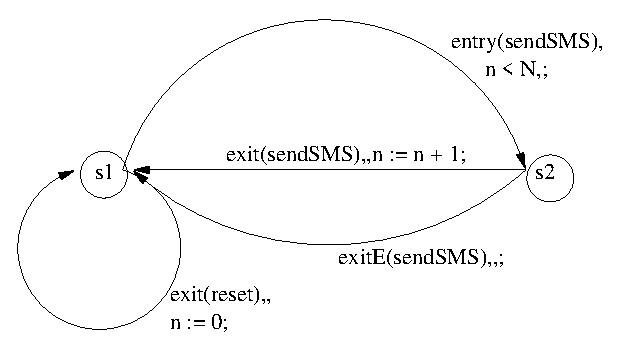
\epsfig{file=limited_sms_alt.eps, width=6cm}
\end{center}
\caption{Example Security Automaton}\label{FigExample}
\end{figure}

Throughout this paper, we will use a simple example property to
illustrate the different translations: the method \texttt{sendSMS} can
be called and terminate successfully at most \(N\) times in between
calls to a \texttt{reset} method (notice that the counter is not
increased upon exceptional termination of
\texttt{sendSMS}, and that we assume that \texttt{reset} cannot be
called from within \texttt{sendSMS}). Figure~\ref{FigExample} shows a
security automaton that can be used to monitor this property (where
\(\varepsilon\) denotes an empty action list). Even though very basic,
this example is representative of a wide range of important
resource-related security properties.

The remainder of this paper is organised as follows.
Section~\ref{SecMVA} formalises the automaton format that we
use and defines the completion function. Next,
Section~\ref{SecProgram} defines the semantics of monitored and
annotated programs. Then Section~\ref{SecAnnotGen} presents the
different translations and proves their
correctness. Section~\ref{SecRelated} discusses related work, while
Section~\ref{SecConcl} concludes and discusses future work.
